\documentclass{beamer}

\beamertemplatenavigationsymbolsempty

\usepackage[utf8]{inputenc}
\usepackage{listings}
\usepackage{minted}
\usepackage{tikz}

\usetikzlibrary{graphs,quotes,arrows.meta}

% set graphics path to figure
\graphicspath{{./figures/}}

\usetheme{Madrid}
\usecolortheme{seahorse}
%Information to be included in the title page:
\title[DataFlowTasks] % optional short title
{DataFlowTasks.jl}

% Custom commands
\newcommand{\DFT}{\texttt{DataFlowTasks.jl}}

\subtitle{Julia \texttt{Task}s which automatically handle data-dependencies}

\author[Faria, Fevotte] % short version of authors
{Luiz~M.~Faria\inst{1} \and François Fevotte\inst{2}}

\institute[]
{
    \inst{1}%
    Chargé de recherche INRIA\\
    POEMS Laboratory
    \and
    \inst{2}%
    FILL ME\\
    FILL ME
}

\date{\today}

\logo{
    
\includegraphics[height=0.5cm]{poems_logo.png}
    % 
\includegraphics[height=0.5cm]{inr_logo_rouge.png}
}

\begin{document}

\frame{\titlepage}

% small textsize on frame
\begin{frame}[fragile]
\frametitle{Overview}

\begin{itemize}
    \item \DFT{} is a Julia package dedicated to parallel programming on multi-core shared memory CPUs.
    \item Automatically infer \texttt{Task} interdependencies based on user annotations (\mintinline{julia}{@R, @W, @RW}).
    \item Heavily inspired by task programming libraries such as StarPU.
    \item Simple API: \mintinline{julia}{@dspawn} macro.
\end{itemize}
%
\begin{columns}[t]
\column{0.3\textwidth}
\begin{exampleblock}{}
\begin{minted}[fontsize=\footnotesize]{julia}
function foo!(A)
  fill!(A, 0)          
  view(A, 1:2) .+= 2   
  view(A, 3:4) .+= 3   
  sum(A)               
end
\end{minted}
\end{exampleblock}
\center 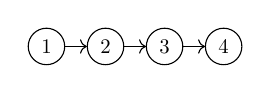
\begin{tikzpicture}[scale=0.75, every node/.style={transform shape}]
\graph[nodes={draw,circle}] {
1 -> 2 -> 3 -> 4
};
\end{tikzpicture}
 
\column{0.6\textwidth}

\begin{exampleblock}{}
\begin{minted}[fontsize=\footnotesize]{julia}
function foo!(A)
  @dspawn fill!(@W(A), 0)         # task 1
  @dspawn @RW(view(A, 1:2)) .+= 2 # task 2
  @dspawn @RW(view(A, 3:4)) .+= 3 # task 3
  @dspawn sum(@R(A))              # task 4
end
\end{minted}
\end{exampleblock}
\center 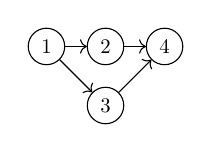
\begin{tikzpicture}[scale=0.75, every node/.style={transform shape}]
\graph[nodes={draw,circle}] {
  1 -> {2, 3} -> 4
};
\end{tikzpicture}

\end{columns}

% In this presentation, we will explore the features and benefits of \DFT{} in the context of efficient parallel programming.

\end{frame}

\begin{frame}
    \frametitle{Table of Contents}
    \tableofcontents
\end{frame}

\section{Introduction}

\subsection{Task based parallelism in Julia}

\begin{frame}[fragile]
\frametitle{Task based parallelism}
\begin{itemize}
    \item A task is a unit of execution or a unit of work
    \item \mintinline{julia}{Task} objects can be created using \mintinline{julia}{@task}
    \item Once created, \mintinline{julia}{Task} objects must be scheduled for execution
    \item Usually, \mintinline{julia}{Task}s are created + scheduled using \mintinline
    {julia}{@spawn}
    \item \alert{Responsibility of synchronizing tasks is left to the programmer}
\end{itemize}

\begin{columns}
\column{0.7\textwidth}    

\begin{example}[Synchronizing tasks]
\begin{minted}{julia}    
A = rand(4)
t1 = @spawn fill!(A,0)
t2 = @spawn (wait(t1); view(A,1:2) += 2)
t3 = @spawn (wait(t1); view(A,3:4) += 3)
t4 = @spawn (wait(t2); wait(t3); sum(A))
fetch(t4)
\end{minted}
\end{example}

\column{0.2\textwidth}

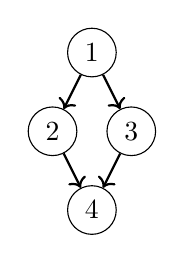
\begin{tikzpicture}
    % Nodes
    \node[circle, draw] (1) at (0, 0) {1};
    \node[circle, draw] (2) at (-0.5, -1) {2};
    \node[circle, draw] (3) at (0.5, -1) {3};
    \node[circle, draw] (4) at (0, -2) {4};
    % Edges
    \draw[->, thick] (1) -- (2);
    \draw[->, thick] (1) -- (3);
    \draw[->, thick] (2) -- (4);
    \draw[->, thick] (3) -- (4);
\end{tikzpicture}

\end{columns}

\end{frame}

\subsection{Motivation}

\begin{frame}[fragile]
\frametitle{Motivation}

\begin{itemize}
    \item Many algorithms make constant re-use of data for efficiency. 
    % \begin{itemize}
    %     \item Merge sort
    %     \item In-place matrix factorization
    %     \item ...
    % \end{itemize}
    \item Reasoning about \mintinline{julia}{Task} interdependencies can be challenging.
    \item Sometimes, simpler to reason about how \mintinline{julia}{Task}s depends on data than how \mintinline{julia}{Task}s depend on each other
\end{itemize}

\begin{example}[Synchronizing tasks]
\begin{minted}[fontsize=\small]{julia}    
A = rand(4)
t1 = @spawn fill!(A,0)                   # RW access to A
t2 = @spawn (wait(t1); view(A,1:2) += 2) # RW access to A[1:2]   
t3 = @spawn (wait(t1); view(A,3:4) += 3) # RW access to A[3:4]
t4 = @spawn (wait(t2); wait(t3); sum(A)) # R access to A
fetch(t4)
\end{minted}
\end{example}

\end{frame}

\subsection{Basic idea}

\begin{frame}[fragile,t]
\frametitle{Basic idea}
\begin{enumerate}
    \item Extract data dependency from user annotations
    \item \textcolor{lightgray}{Infer task dependency from data dependency}
    \item \textcolor{lightgray}{Schedule tasks with inferred dependencies}
\end{enumerate}

\vspace{20pt}
\begin{columns}

\column{0.45\textwidth}    

\begin{minted}[fontsize=\footnotesize]{julia}    
A = rand(4)
@dspawn fill!(@R(A),0)          
@dspawn (@RW(view(A,1:2)) += 2) 
@dspawn (@RW(view(A,3:4)) += 3) 
@dspawn (sum(@R(A))) 
\end{minted}

\column{0.5\textwidth}

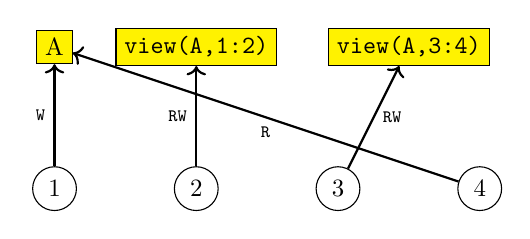
\begin{tikzpicture}[scale=0.9, every node/.style={transform shape}]
    % Nodes
    \node[circle, draw] (1) at (0, 0) {1};
    \node[circle, draw] (2) at (2, 0) {2};
    \node[circle, draw] (3) at (4, 0) {3};
    \node[circle, draw] (4) at (6, 0) {4};
    \node[rectangle, draw, fill=yellow] (A) at (0, 2) {A};
    \node[rectangle, draw, fill=yellow] (A1) at (2, 2) {\texttt{view(A,1:2)}};
    \node[rectangle, draw, fill=yellow] (A2) at (5, 2) {\texttt{view(A,3:4)}};
    
    % Edges
    \draw[->, thick] (1) -- node[midway, left] {\scriptsize \texttt{W}} (A);
    \draw[->, thick] (2) -- node[midway, left] {\scriptsize \texttt{RW}} (A1);
    \draw[->, thick] (3) -- node[midway, right] {\scriptsize \texttt{RW}} (A2);
    \draw[->, thick] (4) -- node[midway, below] {\scriptsize \texttt{R}} (A);
\end{tikzpicture}


\end{columns}

\end{frame}   

\begin{frame}[fragile]

\frametitle{Basic idea}
\begin{enumerate}
    \item \textcolor{lightgray}{Extract data dependency from user annotations}
    \item Infer task dependency from data dependency
    \item \textcolor{lightgray}{Schedule tasks with inferred dependencies}
\end{enumerate}

\center
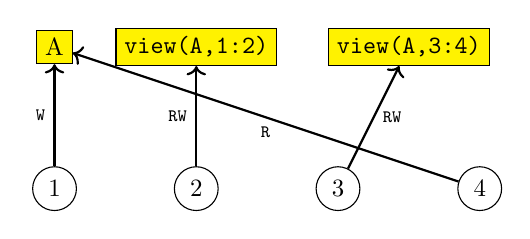
\begin{tikzpicture}[scale=0.9, every node/.style={transform shape}]
    % Nodes
    \node[circle, draw] (1) at (0, 0) {1};
    \node[circle, draw] (2) at (2, 0) {2};
    \node[circle, draw] (3) at (4, 0) {3};
    \node[circle, draw] (4) at (6, 0) {4};
    \node[rectangle, draw, fill=yellow] (A) at (0, 2) {A};
    \node[rectangle, draw, fill=yellow] (A1) at (2, 2) {\texttt{view(A,1:2)}};
    \node[rectangle, draw, fill=yellow] (A2) at (5, 2) {\texttt{view(A,3:4)}};
    
    % Edges
    \draw[->, thick] (1) -- node[midway, left] {\scriptsize \texttt{W}} (A);
    \draw[->, thick] (2) -- node[midway, left] {\scriptsize \texttt{RW}} (A1);
    \draw[->, thick] (3) -- node[midway, right] {\scriptsize \texttt{RW}} (A2);
    \draw[->, thick] (4) -- node[midway, below] {\scriptsize \texttt{R}} (A);
\end{tikzpicture}

\begin{exampleblock}{}
\centering    
\begin{minted}[fontsize=\footnotesize]{julia}
for i in 1:N, j in i:-1:1
  # detect conflict between i and j
  for di in data(i), dj in data(j)
    memory_overlap(di,dj) && add_edge(j,i)
  end
end
\end{minted}    
\end{exampleblock}

% \alert{Note the quadratic complexity in the number of tasks!}

\end{frame}

\begin{frame}[fragile]

    \frametitle{Basic idea}
    \begin{enumerate}
        \item \textcolor{lightgray}{Extract data dependency from user annotations}
        \item \textcolor{lightgray}{Infer task dependency from data dependency}
        \item Schedule tasks with inferred dependencies
    \end{enumerate}
    
    \center
    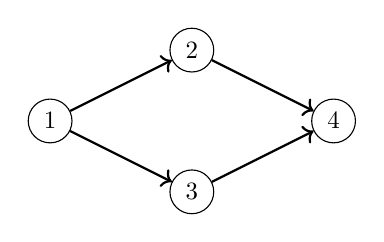
\begin{tikzpicture}[scale=0.9, every node/.style={transform shape}]
        % Nodes
        \node[circle, draw] (1) at (0, 0) {1};
        \node[circle, draw] (2) at (2, 1) {2};
        \node[circle, draw] (3) at (2, -1) {3};
        \node[circle, draw] (4) at (4, 0) {4};
        
        % Edges
        \draw[->, thick] (1) -- (2);
        \draw[->, thick] (1) -- (3);
        \draw[->, thick] (2) -- (4);
        \draw[->, thick] (3) -- (4);
    \end{tikzpicture}
    
\begin{exampleblock}{}
\centering    
\begin{minted}[fontsize=\footnotesize]{julia}
for i in 1:N
  deps = inneighbors(i)
  for j in deps
    wait(j)
  end
  schedule(i)
end
\end{minted}    
\end{exampleblock}
    
    % \alert{Note the quadratic complexity in the number of tasks!}
    
\end{frame}

\section{\mintinline{julia}{Implementation details}}

\subsection{\mintinline{julia}{DataFlowTask}}

\begin{frame}[fragile]

\frametitle{\texttt{DataFlowTask}: \mintinline{julia}{@dspawn} macro}

The \mintinline{julia}{@dspawn} macro does the following:

\begin{itemize}
    \item Scan the \mintinline{julia}{Expr} for \mintinline{julia}{@R, @W, @RW} annotations
    \item Create a \mintinline{julia}{data} and \mintinline{julia}{access_mode}
    tuple
    \item Remove annotations from the \mintinline{julia}{Expr}
    \item Parse keyword arguments    
    \item Create an anonymous function wrapping the new \mintinline{julia}{Expr}
    \item Insert a call to \mintinline{julia}{DataFlowTask} constructor
\end{itemize}

\begin{columns}

\column{0.4\textwidth}    
\begin{exampleblock}{}    
\begin{minted}{julia}
@dspawn begin
  @RW A
  @R B
  A .= A .+ B
end label="add(A,B)"
\end{minted}
\end{exampleblock}

\column{0.5\textwidth}    

\begin{exampleblock}{}    
\begin{minted}{julia}
DataFlowTasks((A,B),(RW,R);
  label="add(A,B)") do 
  A .= A .+ B
end 
\end{minted}
\end{exampleblock}

\end{columns}
%

\end{frame} 

\begin{frame}[fragile]

\frametitle{\texttt{DataFlowTask} structure}

\small{\alert{Inner-constructor of \mintinline{julia}{DataFlowTask} handles much of
the insertion/removal logic:}}

\hrulefill
\begin{minted}[fontsize=\footnotesize]{julia}
mutable struct DataFlowTask
  data::Tuple
  access_mode::NTuple{<:Any,AccessMode}
  task::Task
  ...
  function DataFlowTask(f,data,mode,taskgraph)
    tj = new(data, mode) # incomplete initialization
    addnode!(taskgraph, tj, true) 
    deps = inneighbors(taskgraph, tj) |> copy
    tj.task = @task do
      foreach(ti->wait(ti),deps)
      res = f() # run the underlying function
      put!(taskgraph.finished, tj)
      return res
    end
  end
end
\end{minted}

\end{frame} 

\subsection{\mintinline{julia}{DAG}}

\begin{frame}[fragile]
\frametitle{{\mintinline{julia}{DAG}}}  

A graph data structure to store \mintinline{julia}{DataFlowTask}s and their
dependencies:

\begin{itemize}
  \item Dynamic: nodes are added and removed on the fly
  \item Buffered: limit the number of active nodes
  \item Thread-safe: multiple threads can add/remove nodes
  \item Efficient: easy access to both in- and out-neighbors
\end{itemize}

\hrulefill
\begin{minted}[fontsize=\footnotesize]{julia}
struct DAG{T}
  inoutlist::OrderedDict{T,Tuple{Set{T},Set{T}}}
  cond_push::Condition
  cond_empty::Condition
  lock::ReentrantLock
  sz_max::Base.RefValue{Int}
  counter::Base.RefValue{Int}
  _buffer::Set{Int} # used for transitive reduction
end
\end{minted}
  
\end{frame}

\subsection{\mintinline{julia}{TaskGraph}}

\begin{frame}[fragile]
\frametitle{{\mintinline{julia}{Taskgraph}}}  
  
Essentially a \mintinline{julia}{DAG{DataFlowTask}} with
\begin{itemize}
  \item A channel to store finished tasks  
  \item A dedicated \mintinline{julia}{Task} to remove nodes from the graph
\end{itemize}

\hrulefill
\begin{minted}[fontsize=\footnotesize]{julia}
mutable struct TaskGraph
  dag::DAG{DataFlowTask}
  finished::FinishedChannel{Stoppable{DataFlowTask}}
  dag_cleaner::Task
  function TaskGraph(sz = typemax(Int))
    dag = DAG{DataFlowTask}(sz)
    finished = FinishedChannel{Stoppable{DataFlowTask}}()
    tg = new(dag, finished)
    start_dag_cleaner(tg)
    return tg
  end
end
\end{minted}

\begin{alertblock}{}
\small{Recall that \mintinline{julia}{DataFlowTask} inserts itself in the task
graph, and its underlying \mintinline{julia}{Task} moves it into the finished
channel.}
\end{alertblock}
  
\end{frame}

\subsection{Logging}

\begin{frame}
\frametitle{Logging}

To help with debugging and performance analysis, \DFT{} provides some logging
and visualization tools:
\begin{itemize}
  \item Use the \mintinline{julia}{@log} macro to log the execution of block
  \item Once logged, \mintinline{julia}{describe(loginfo)} shows a summary
  \item If \mintinline{julia}{GraphViz} is installed,
  \mintinline{julia}{Graph(loginfo)} displays the \mintinline{julia}{DAG}
  \item If \mintinline{julia}{Makie} is available,
  \mintinline{julia}{plot(loginfo)} plots the execution trace
\end{itemize}

The basic logic of logging is as follows:
\begin{itemize}
  \item Create a \mintinline{julia}{LogInfo} object is created at the start of the block  
  \item Overwrite the function
  \mintinline{julia}{should_log()} to return \mintinline{julia}{true}
  \item Create tasks. When tasks are created, they check
  \mintinline{julia}{should_log()} and log their execution as well as the
  \mintinline{julia}{DAG} structure
  \item Set \mintinline{julia}{should_log()} to \mintinline{julia}{false}
\end{itemize}

\begin{alertblock}{}
  Note: because \mintinline{julia}{should_log()} is a simple pure function,
  logging should have zero overhead when disabled.
\end{alertblock}

\end{frame}

\begin{frame}[fragile]
\frametitle{Logging}

\begin{minted}[fontsize=\footnotesize]{julia}
function work(A, B)
    @dspawn init!(@W(A))               label="init A"
    @dspawn init!(@W(B))               label="init B"
    @dspawn mutate!(@RW(A))            label="mutate A"
    @dspawn mutate!(@RW(B))            label="mutate B"
    res = @dspawn result(@R(A), @R(B)) label="read A,B"
    fetch(res)
end
log_info = DataFlowTasks.@log work(A, B)
DataFlowTasks.describe(log_info; categories=["init", "mutate", "read"])

\end{minted}

\center 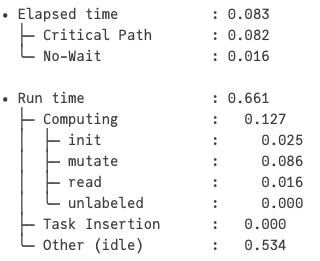
\includegraphics[width=0.3\textwidth]{figures/unicode-output.png}
  
\end{frame}

\begin{frame}[fragile]
\frametitle{Logging}

\begin{minted}[fontsize=\footnotesize]{julia}
function work(A, B)
  @dspawn init!(@W(A))               label="init A"
  @dspawn init!(@W(B))               label="init B"
  @dspawn mutate!(@RW(A))            label="mutate A"
  @dspawn mutate!(@RW(B))            label="mutate B"
  res = @dspawn result(@R(A), @R(B)) label="read A,B"
  fetch(res)
end
using GraphViz
GraphViz.Graph(log_info)
  
\end{minted}
  
\center 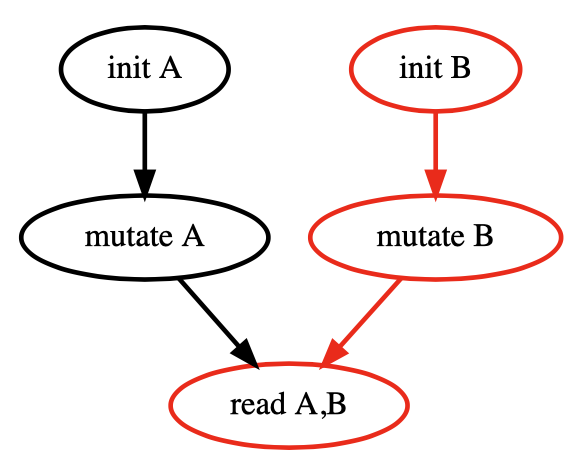
\includegraphics[width=0.3\textwidth]{figures/dag-output.png}
    
\end{frame}

\begin{frame}[fragile]
\frametitle{Logging}

\begin{minted}[fontsize=\footnotesize]{julia}
function work(A, B)
  @dspawn init!(@W(A))               label="init A"
  @dspawn init!(@W(B))               label="init B"
  @dspawn mutate!(@RW(A))            label="mutate A"
  @dspawn mutate!(@RW(B))            label="mutate B"
  res = @dspawn result(@R(A), @R(B)) label="read A,B"
  fetch(res)
end
using CairoMakie # or GLMakie to benefit from more interactivity
plot(log_info; categories=["init", "mutate", "read"])
    
  \end{minted}
    
  \center 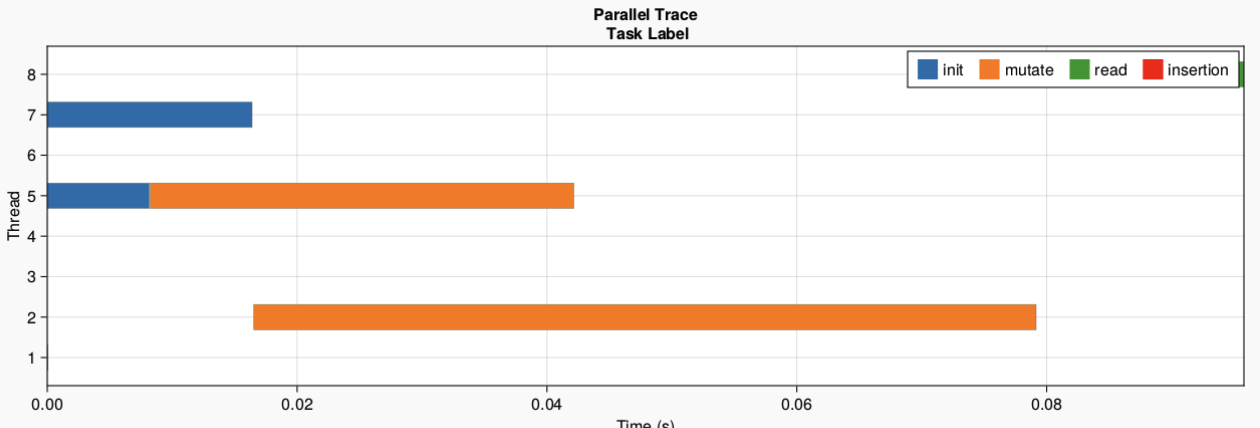
\includegraphics[width=0.8\textwidth]{figures/trace-output.png}
      
  \end{frame}

\subsection{Summary}

\begin{frame}
\frametitle{Summary}  

\begin{itemize}
  \item When \DFT{} is loaded a default \mintinline{julia}{TaskGraph}, with an
  internal \mintinline{julia}{DAG}, is instantiated.
  \item Upon creation, each \mintinline{julia}{DataFlowTask} object inserts
  itself in the task graph.
  \item Upon completion, each \mintinline{julia}{DataFlowTask} object inserts
  itself in a finished channel
  \item An asynchronous task is responsible for removing finished jobs from the graph
  \item The \mintinline{julia}{@dspawn} macro provides a very convenient way to
  create \mintinline{julia}{DataFlowTask}s
  \item Logging is enabled using the \mintinline{julia}{@log} macro
\end{itemize} 
\end{frame}

\section{Live examples}

\begin{frame}{Live examples}
  \begin{itemize} 
    \item \href{https://maltezfaria.github.io/DataFlowTasks.jl/dev/examples/cholesky/cholesky/}{Tiled cholesky factorization}
    \item
    \href{https://maltezfaria.github.io/DataFlowTasks.jl/dev/examples/blur-roberts/blur-roberts/}{Blur-Roberts filter}
    \item
    \href{https://maltezfaria.github.io/DataFlowTasks.jl/dev/examples/lcs/lcs/}{Longest
    common subsequence}
    \item
    \href{https://maltezfaria.github.io/DataFlowTasks.jl/dev/examples/sort/sort/}{Merge sort}
  \end{itemize}
\end{frame}

\section{Roadmap}


\end{document}